\documentclass[letterpaper, 12pt]{article}
\usepackage{mathtools}
\DeclarePairedDelimiter\abs{\lvert}{\rvert}     %serve per mettere il modulo 
\usepackage{booktabs}
\usepackage{bm}
\usepackage{textcomp}
\usepackage{colortbl}
\usepackage{tabularx}
\usepackage{siunitx}
\usepackage{enumitem}
\usepackage{xcolor}
\usepackage{fancyhdr}
\usepackage{caption}
\usepackage{changepage}
\usepackage{amsmath} 
\usepackage{subcaption}
\usepackage{graphicx}
\usepackage[table]{xcolor} 
\usepackage[margin=1in,letterpaper]{geometry} % decreases margins
\usepackage{cite} % takes care of citations
\usepackage[hidelinks]{hyperref} % adds hyper links inside the generated pdf file
\usepackage{blindtext}

% Setup hyperref
\hypersetup{
    colorlinks=false, % colored links
    linkcolor=linkcolor, % color for internal links
    citecolor=citecolor, % color for citations
    urlcolor=urlcolor, % color for URLs
}
\fancypagestyle{logoheader}{
    \fancyhf{}
    \fancyhead[L]{
\includegraphics[width = 3cm]{logo_bicocca.png}}
    \renewcommand{\headrulewidth}{0pt}
}
\setlength{\headheight}{72.63475pt} % Fix fancyhdr warning
\addtolength{\topmargin}{-0.75pt} % Compensate for increased headheight

\graphicspath{{immagini/}}
%Required for inserting images
%++++++++++++++++++++++++++++++++++++++++
%Margini 


\begin{document}


\title{{\small Università degli studi Milano Bicocca - Dipartimento di Fisica}\\
	Esperimentazioni di Fisica Computazionale}
\author{S. Franceschina}
\date{\today}
\maketitle
\thispagestyle{logoheader}

%Abstract da completare
\begin{abstract} 
	\begin{adjustwidth}{-1cm}{-1cm}
	\end{adjustwidth}
\end{abstract}
\tableofcontents
\newpage

\section{Analisi dell'errore}
\subsection{Teoria}
Nella presente sezione analizziamo le due principali fonti di errore in contesti computazionali: 
\begin{enumerate}
    \item Errori di arrotondamento: dovuti alla rappresentazione di numeri reali con numero finito di digits.
    \item Errori di approssimazione: dovuti alla modalità stessa con cui affrontiamo il problema, 
          per questo motivo sono presenti anche nel caso ideale. 
\end{enumerate}

\subsection{Esercizio 1.0.1}
L'esercizio richiede di studiare $f(x)=e^x$ nell'intervallo $[0,1]$, calcolando numericamente il suo sviluppo in 
serie: $g_N(x)=\sum_{n=0}^N \frac{x^n}{n}$

In particolare bisogna mostrare che

\begin{equation}
    \Delta=|f(x)-g_N(x)| \approx \frac{x^{N+1}}{(N+1)!}
\end{equation}

Al fine dell'esercizio vengono rappresentati nel grafico \ref{fig:es1_0_1_1} le funzioni $\Delta$ e $\frac{x^{N+1}}{(N+1)!}$, con 
$N=1,2,3, 4$, al variare di $x$ nell'intervallo $[0,1]$. 

\begin{figure}[ht!]
    \centering
    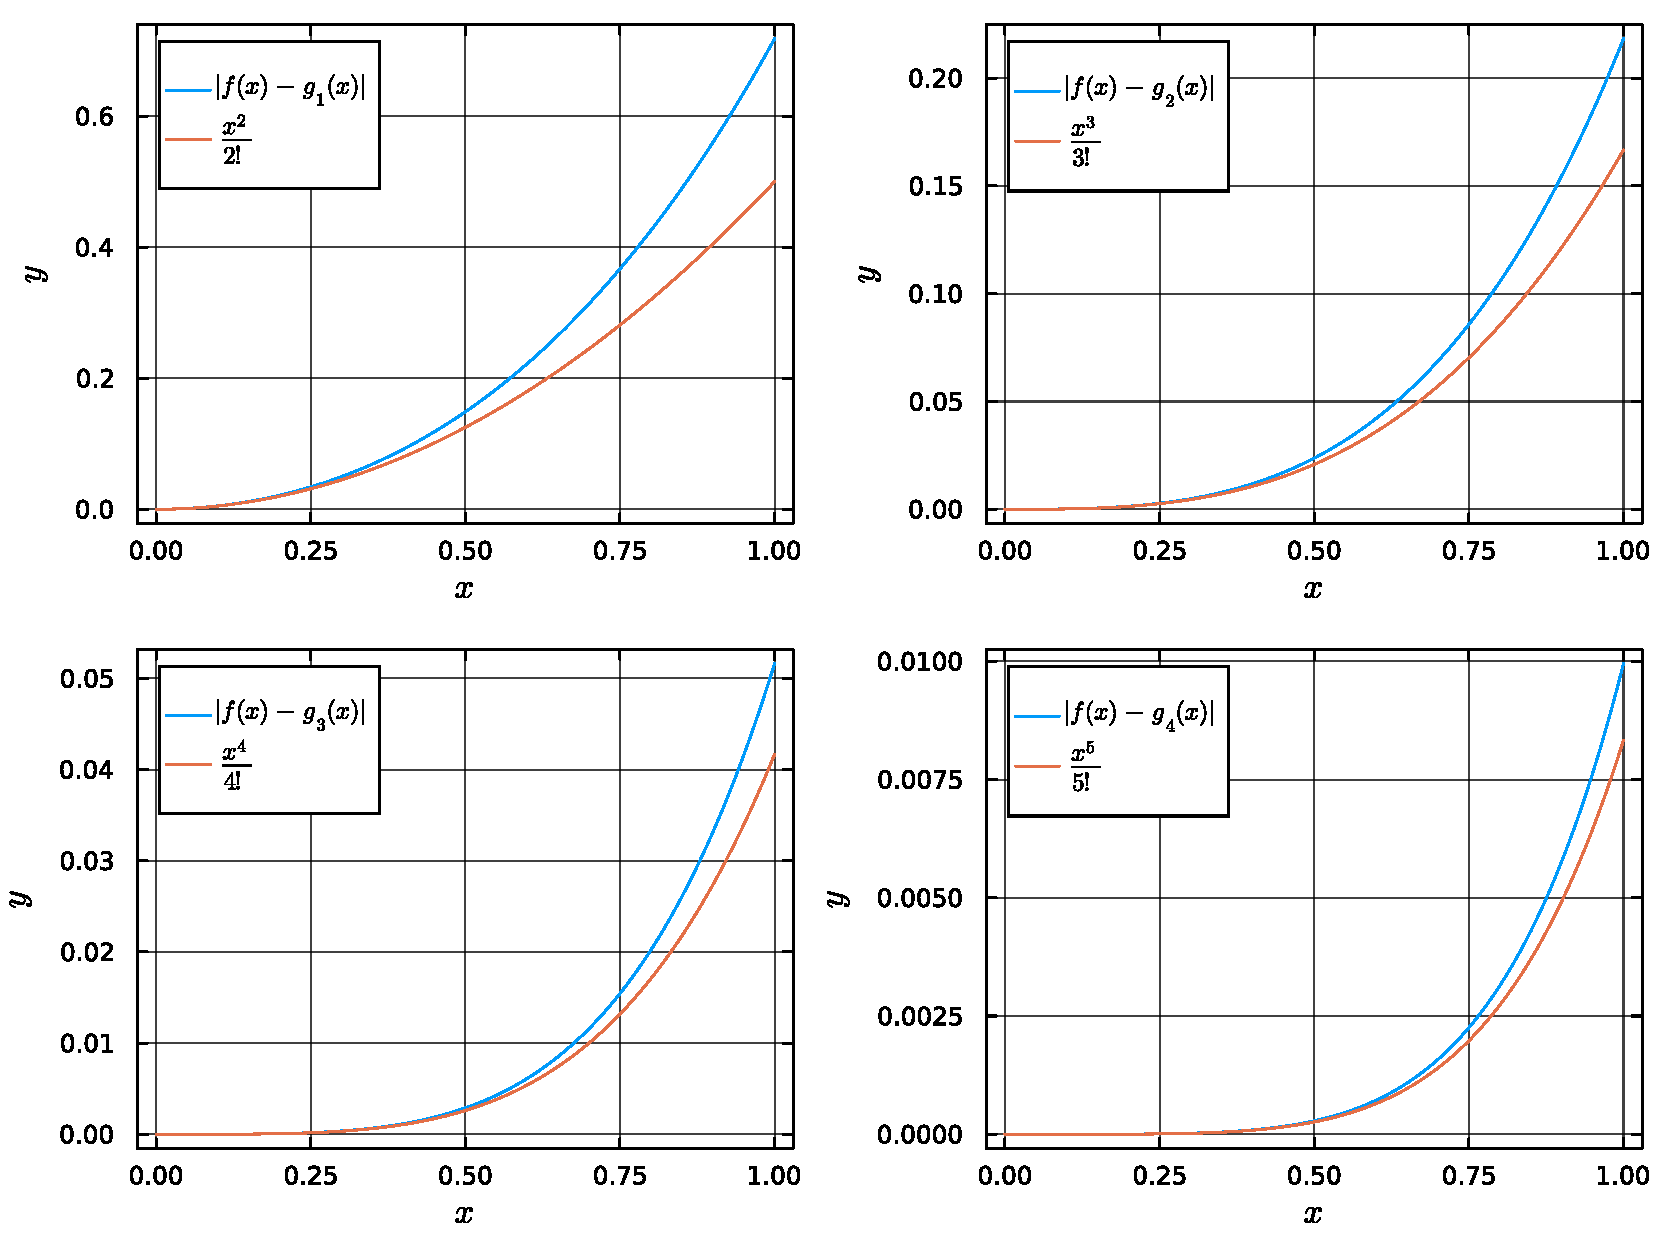
\includegraphics[width=0.8\textwidth]{1011.pdf}
    \caption{Confronto tra $\Delta$ e $\frac{x^{N+1}}{(N+1)!}$ per $N=1,2,3, 4$.}
    \label{fig:es1_0_1_1}
\end{figure}

La prima considerazione che possiamo fare è che all'aumentare di $N$ la funzione $\Delta$ 
assume valori sempre più vicini allo zero. Questo significa che la distanza tra il valore 
della funzione $f(x)$ presa in esame e la sua espansione di Taylor troncata all'ordine 
$N$ diminuisce. In effetti ci aspettiamo che la funzione $\Delta$ sia 
esattamente zero nel caso in cui $N \rightarrow \infty$. Inoltre possiamo notare che la funzione $\Delta$, in ognuno
dei grafici, è tanto più prossima allo zero quanto più ci si avvicina all'origine, poichè l'espansione in serie 
richiede $x \rightarrow 0$.\\
La seconda considerazione è che le funzioni $\Delta$ e $\frac{x^{N+1}}{(N+1)!}$ si 
avvicinano tra loro all'aumentare di $N$. Questo risponde alla richiesta dell'esercizio, 
cioè che l'errore scali come un polinomio di ordine $N+1$. 

\subsection{Esercizio 1.2.1}


\section{Sistemi lineari}
\subsection{Teoria}

\section{Radici di equazioni non lineari}
\subsection{Teoria}

\section{Interpolazioni}
\subsection{Teoria}

\section{Integrazione numerica}
\subsection{Teoria}

\section{Equazioni differenziali ordinarie}
\subsection{Teoria}

\end{document}